\documentclass[10pt,a4paper]{IEEEtran}
\usepackage[utf8]{inputenc}
\usepackage[spanish]{babel}
\usepackage{amssymb}
\usepackage{graphicx}
\usepackage{float}
\usepackage{hyperref}
\usepackage{subcaption} 
\usepackage{amsmath}
\usepackage{amsfonts}
\usepackage[usenames]{color}

\begin{document}
\title{Laboratorio 2}
\author{\IEEEauthorblockN{Nombre\IEEEauthorrefmark{2}$^1$ y G. Millain\IEEEauthorrefmark{2}$^2$\vspace{0.2cm}}\IEEEauthorblockA{\IEEEauthorrefmark{2}\emph{Facultad de Ingeniería, Universidad Nacional del Comahue}\\\emph{Buenos Aires 1400, 8300 Neuquén}}\IEEEauthorblockA{$^1$\texttt{\small{mail}}\\$^2$\texttt{\small{gonza.pm@outlook.com}}}}

\maketitle

\begin{abstract}
    Se empieza por analizar cada uno de los bloques que conforma una malla de fase encadenada (PLL). Luego se observa su uso a la hora de demodular una señal FM. 
\end{abstract}
\section{Procedimiento a seguir}
\begin{itemize}
	\item Frecuencia libre de $V_{CO}$ cuando $V_{in}=0V$.
	\item Frecuencia libre vs variaciones de R=1k %poner R_{1} / R_{2} segun corresponda
	\item Frecuencia libre vs $R$ y $\tau$
	\item llevar la salida del $V_{CO}$ a $8KHz$ con $in_2$ en $1KHz$.
	\item Conectar el generador a una frecuencia que el PLL enganche %entre 500Hz y 1.5KHz
	\item Salida de $V_{CO}$
	\item Variacion de la frecuencia del generador de entrada
	\item Calculo de $f_c$ del circuito RC.
	\item Variaciones de $C$.
	\item Medicion de $C$ para frecuencias de enganche superior e inferior y para 1KHz de entrada 
	\item Medicion de $C$ para frecuencias de $4kHz, 5KHz, 6KHz$.
\end{itemize}

    \section{Marco teórico}
    \subsection{Detector de fase}
    Un detector de fase es un mezclador optimizado para usarse con frecuencias de entrada iguales. También se lo denomina detector de fase, dado que la cantidad de voltaje de CD depende del ángulo de fase $\phi$ entre las señales de entrada.
    
    Se muestra la función del detector de fase a partir de dos señales senoidales en la Fig. \ref{def1}.
    
    \begin{figure}[H]
        \centering
        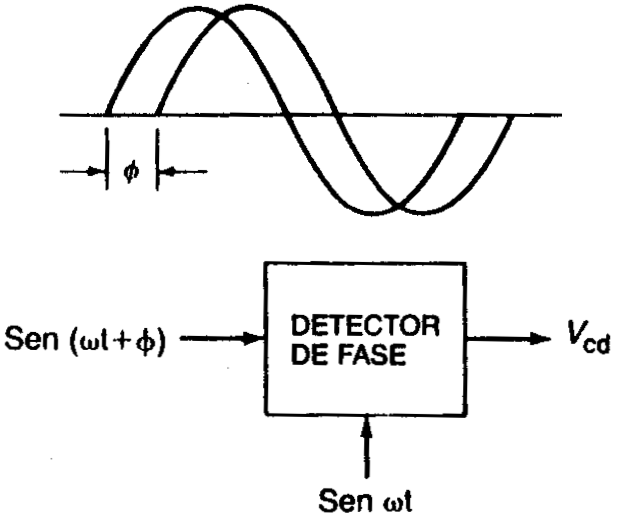
\includegraphics[scale=0.3]{def1.png}
        \caption{Funciones de entrada y diagrama en bloque.}
        \label{def1}
    \end{figure}
    
    Cuando el ángulo de fase $\phi=0$, el voltaje de CD es máximo. A medida que el ángulo de fase se incrementa de $0$\textordmasculine  a $180$\textordmasculine, el voltaje de cd decrece a su valor mínimo. Cuando $\phi=90$\textordmasculine, la salida de CD es el promedio entre la salida máxima y mínima. Una grafica de la función a la salida se muestra en la Fig. \ref{def2}.
    
    \begin{figure}[H]
        \centering
        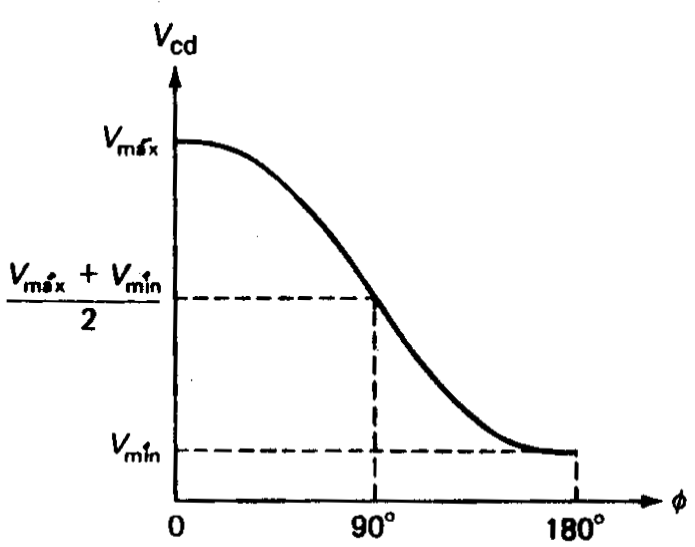
\includegraphics[scale=0.3]{def2.png}
        \caption{Salida del detector de fase}
        \label{def2}
    \end{figure}
    
    \subsection{Oscilador controlado por voltaje (VCO)}
    En un VCO, un voltaje de CD de entrada controla la frecuencia de salida, como se muestra en la Fig. \ref{vco1}.
    
    \begin{figure}[H]
        \centering
        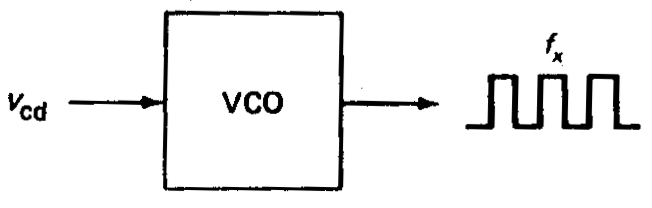
\includegraphics[scale=0.3]{vco1.png}
        \caption{Diagrama en bloque del VCO.}
        \label{vco1}
    \end{figure}
    
    Un voltaje de CD controla la frecuencia del oscilador. Típicamente la frecuencia decrece en forma lineal con un incremento en el voltaje de CD, como se muestra en la Fig. \ref{vco2}.
    
    \begin{figure}[H]
        \centering
        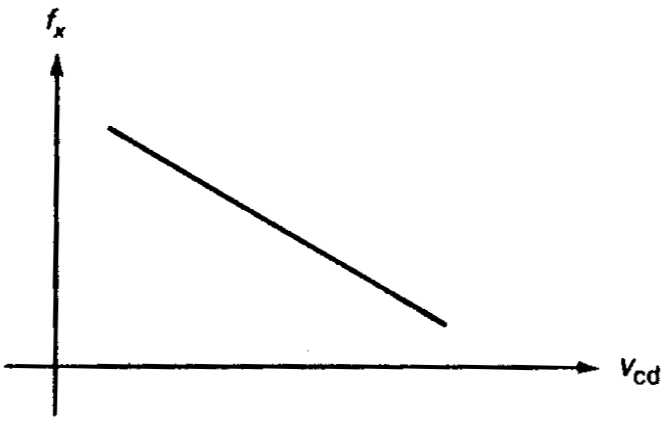
\includegraphics[scale=0.3]{vco2.png}
        \caption{Relación voltaje de CD y frecuencia de salida.}
        \label{vco2}
    \end{figure}
    
    \subsection{Malla de fase encadenada (PLL)}
    En un PLL \emph{(phase-locked-loop)}; son entradas al detector de fase una señal con frecuencia $f_x$, y otra proveniente de un VCO. La señal de salida del detector pasa por un filtro pasabajos, que remueve las frecuencias originales, sus armónicas y la frecuencia suma. Por lo tanto queda la frecuencia diferencia (voltaje de CD) a la salida del filtro. Este voltaje de CD controla la frecuencia del VCO. En la Fig. \ref{pll1} se muestra el diagrama en bloque del PLL.
    
    \begin{figure}[H]
        \centering
        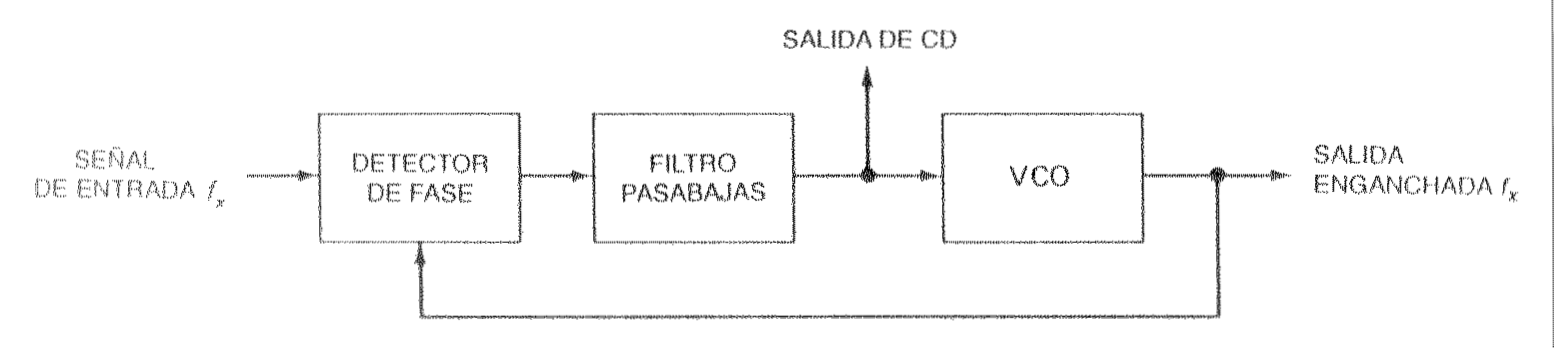
\includegraphics[scale=0.2]{pll1.png}
        \caption{Diagrama en bloque del PLL.}
        \label{pll1}
    \end{figure}
    %%
    El sistema realimentado “engancha” la frecuencia del VCO a la frecuencia de entrada. Cuando el sistema trabaja de manera correcta, la frecuencia a la salida del VCO es igual a $f_x$, igual a la señal de entrada. Por lo tanto, el 
    detector de fase tiene dos entradas con frecuencias iguales; el ángulo de fase entre estas entradas determina la cantidad de voltaje de cd de salida. 
    
    \begin{figure}[H]
        \centering
        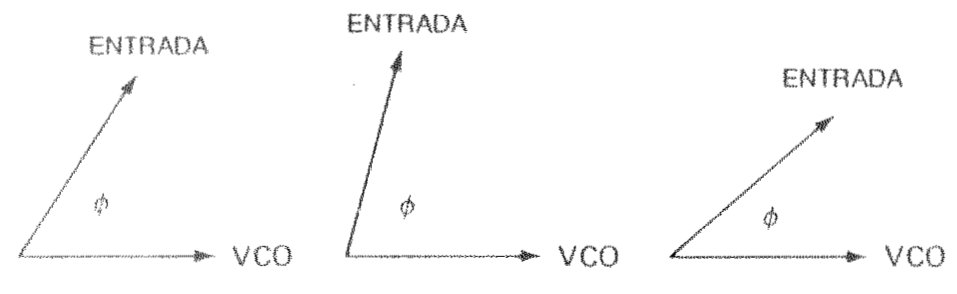
\includegraphics[scale=0.3]{pll2.png}
        \caption{Fasores de la señal de entrada y VCO.}
        \label{pll2}
    \end{figure}
    
    Los fasores para la señal de entrada y la del VCO se muestran en la Fig. \ref{pll2}. Si la frecuencia de entrada cambia, la frecuencia del VCO la seguirá. 
    
    Por ejemplo, si la frecuencia de entrada $f_x$ se incrementa, su fasor gira más rápido y el ángulo de fase aumenta. Esto significa que saldrá menos voltaje de cd en la salida del detector de fase. El voltaje de cd más bajo forzara a que la frecuencia del VCO se incremente hasta que se iguala a la frecuencia de entrada.
    
    Por otro lado, si la frecuencia de entrada decrece, su fasor disminuye su velocidad de giro y el ángulo de fase decrece. Se tiene más voltaje de cd a la salida del detector de fase, lo cual causa que la frecuencia del VCO disminuya hasta que se iguala a la frecuencia de entrada.
    
    \subsection{Intervalo de enganche}
    El intervalo de enganche $B_L$ es el intervalo de frecuencias que el VCO puede producir, dado por 
    
    \begin{equation}\label{bl}
    B_L = f_{max}-f_{min} 
    \end{equation}
    
    Donde $f_{max}$ y $f_{min}$ son las frecuencias máxima y mínima del VCO.
    Cuando $f_x$ se encuentra dentro de este intervalo, el VCO seguirá esta frecuencia de entrada y la frecuencia de salida será igual a $f_x$.
    
    \subsection{Funcionamiento libre}
    Si la señal de entrada se desconecta, el VCO oscila en modo de funcionamiento libre a una frecuencia que determinan las componentes del circuito. 
    
    \subsection{Captura y enganche}
    Si la PLL esta en funcionamiento libre, esta se 
    puede enganchar a la frecuencia de entrada cuando la frecuencia de entrada cae dentro del intervalo de captura $B_C$, una banda de frecuencias centrada alrededor de la frecuencia de funcionamiento libre; dado por.
    
    \begin{equation}\label{bc}
    B_C = f_{2}-f_{1} 
    \end{equation}
    
    Donde $f_{1}$ y $f_{2}$ son las frecuencias entre las que el PLL se puede enganchar. Este intervalo siempre es menor o igual al intervalo de enganche y esta relacionado con la frecuencia de corte del filtro pasa-bajo. Mientras la frecuencia de corte es más baja, el intervalo de captura es más pequeño.
    
    \subsection{Salida de FM}
    La Fig. \ref{sal} muestra un simple modulador de FM, compuesto por un oscilador LC con un capacitor de sintonización variable. Al variar la capacitancia, la frecuencia de oscilación cambia.
    
    \begin{figure}[H]
        \centering
        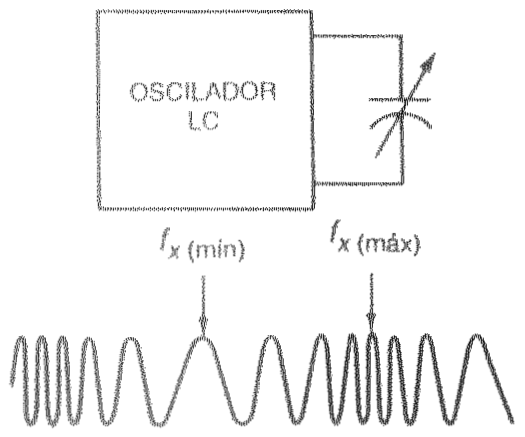
\includegraphics[scale=0.3]{sal.png}
        \caption{Diagrama en bloque modulador de FM.}
        \label{sal}
    \end{figure}
    
    Cuando una señal de FM es la entrada de una PLL, el VCO seguirá la frecuencia de entrada a medida que este cambie. Como resultado, se tiene un voltaje variable a la salida del filtro. Este voltaje tiene la misma frecuencia que la señal 
    moduladora. 
    En resumen la salida de CD representa una salida de FM demodulada.
\section{Desarrollo}
    Para el desarrollo de las actividades propuestas implementamos el circuito en el simulador:
    \begin{figure}[H]
        \centering
        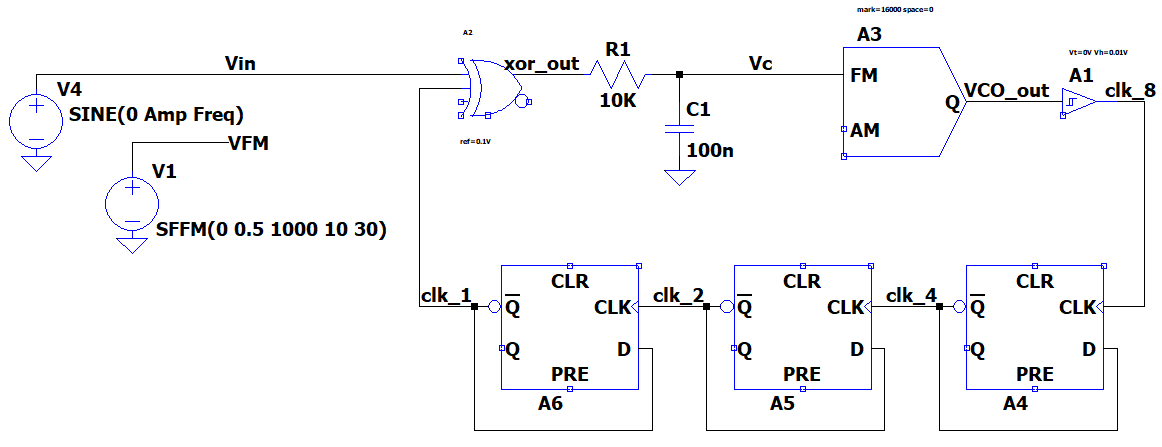
\includegraphics[width=.45\textwidth]{Fig/CircuitoBase}
        \caption{Circuito PLL}
        \label{circuito}
    \end{figure}
Se desconecta la señal de entrada $Vin$ con el fin de medir la frecuencia de operación libre
del PLL. Para esto se hace uso de la herramiento ``FFT'' y se encuentra la frecuencia correspondiente al nodo $clk1$. Dando como resultado que la 
frecuencia de operacion libre es de aproximadamente $980Hz$ para $R1=10K$ y $C1=100n$. El resultado mencionado se observa 
en la figura \ref{Flibre}:
\begin{figure}[H]
    \centering
    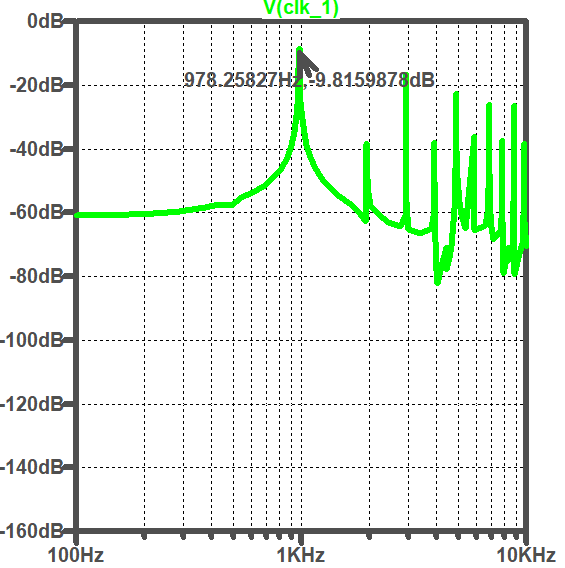
\includegraphics[width=.45\textwidth]{Fig/FrecuenciaLibre_VCO16K_R10K_C100n}
    \caption{FFT de la señal salida de VCO, evidenciando la frecuencia de operación libre}
    \label{Flibre}
\end{figure}
El siguiente paso es realizar un barrido de valores para resistencia $R1$ y ver la variabilidad de la frecuencia libre del PLL. Nuevamente 
hacemos uso de la FFT y vemos el resultado obtenido en la figura \ref{RBarrido}:
\begin{figure}[H]
    \centering
    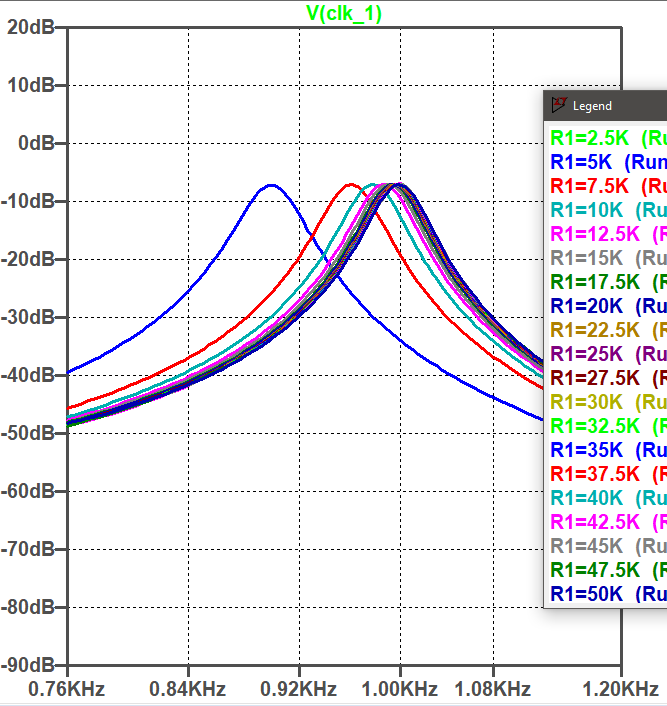
\includegraphics[width=.45\textwidth]{Fig/FrecuenciaLibreVariandoR50K}
    \caption{Frecuencia de operación libre para 20 distintos valores de $R1$}
    \label{RBarrido}
\end{figure}
Se observa que para un rango de valores de $R1$ que parte de $2,5K$ hasta $50K$ con paso de $2,5K$ se obtienen frecuencia de operación libre 
muy cercanas a $1Khz$ y la tendencia es creciente. Con estos valores se calcula el $\tau$ del filtro pasa bajos formado por 
$R1$ y $C1$, registrado en la Tabla \ref{TablaTau}. Se deduce que aumentar la resistencia dejando fijo el valor de $C1$ genera un aumento 
en la frecuencia libre pero tambien en el tiempo que requiere el sistema para engancharse ($\tau$).\\
%AGREGAR TABLA
Con el fin de obtener a la salida del $VCO$, denotado con $A3$ en la figura \ref{circuito}, una frecuencia de $8Khz$ y por lo tanto en el nodo 
$clk1$ una frecuencia de $1Khz$ (ya que los tres flip flop generan un divisor por 8) se inspecciona la figura \ref{RBarrido}. Vemos que para 
una resistencia de $50K$ la frecuencia libre es igual a $1Khz$ que es lo requerido, por lo tanto a partir de ahora el valor de $R1=50K$.\\
Calculada la frecuencia libre del sistema y viendo como esta varia con $R1$ lo siguiente es analizar el funcionamiento del PPL, para esto conectamos 
la fuente $Vin$ a la XOR y variamos su frecuencia en un rango alrededor de $1Khz$ (frecuencia libre) con el fin de encontrar de forma empírica el rango
de frecuencias para el cual el PLL se engancha. Es decir, el rango de frecuencia que el circuito puede seguir a la señal de entrada. Los resultados obtenidos siguiendo estos 
pasos son:
\begin{itemize}
    \item Frecuencia inferior de engache $F_{Einf} =790Hz$
    \begin{figure}[H]
        \centering
        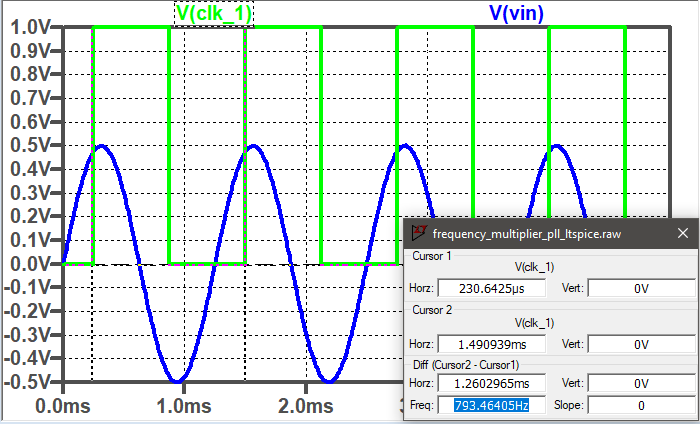
\includegraphics[width=.45\textwidth]{Fig/Engancheinferior}
        \caption{Verde:Señal de entrada de $790Hz$. Azul:Señal de enganche del PLL de $793Hz$ (nodo $clk1$)}
        \label{Einf}
    \end{figure}
    \item Frecuencia media de enganche $F_{Emed}=1KHz$
    \begin{figure}[H]
        \centering
        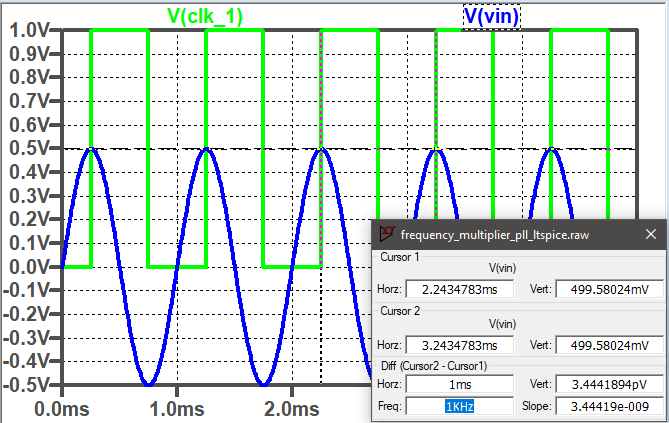
\includegraphics[width=.45\textwidth]{Fig/EngancheMedio}
        \caption{Verde:Señal de entrada de $1KHz$. Azul:Señal de enganche del PLL de $1KHz$ (nodo $clk1$)}
        \label{Emed}
    \end{figure} 
    \item Frecuencia superior de enganche $F_{Esup}=1,2KHz$
    \begin{figure}[H]
        \centering
        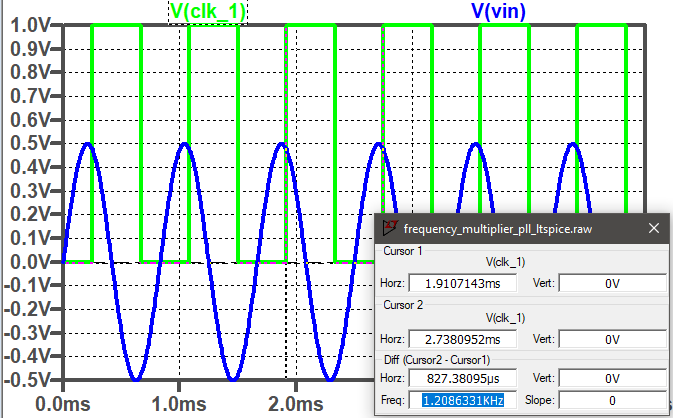
\includegraphics[width=.45\textwidth]{Fig/EngancheSuperior}
        \caption{Verde:Señal de entrada de $1,2KHz$. Azul:Señal de enganche del PLL de $1,2KHz$ (nodo $clk1$)}
        \label{Esup}
    \end{figure}
\end{itemize}  
Como vemos en las figuras \ref{Einf}, \ref{Emed} y \ref{Esup} para un rango de frecuencias $[790Hz,1,2KHz]$ la señal de salida del VCO 
sigue de manera precisa a la señal de entrada (replicando su frecuencia). Por otro lado, en las figuras \ref{NEinf} y \ref{NEsup} vemos que para frecuencias de señal
de entrada de $500Hz$ y $1,5KHz$, respectivamente, el PPL es incapaz de engancharse.
\begin{figure}[H]
    \centering
    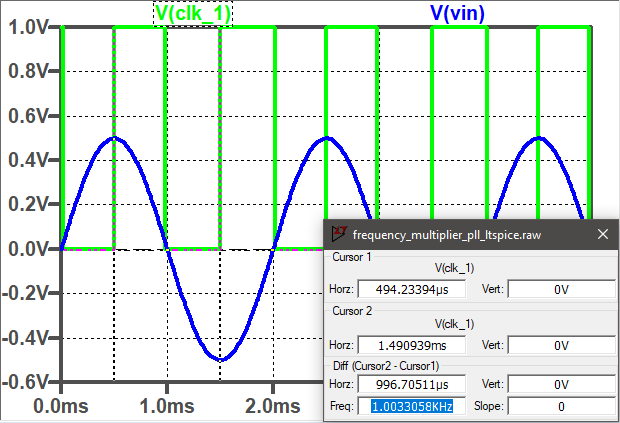
\includegraphics[width=.45\textwidth]{Fig/NoEnganche500}
    \caption{Verde:Señal de entrada de $500Hz$. Azul:Señal de enganche del PLL de $1KHz$ (nodo $clk1$)}
    \label{NEinf}
\end{figure}
\begin{figure}[H]
    \centering
    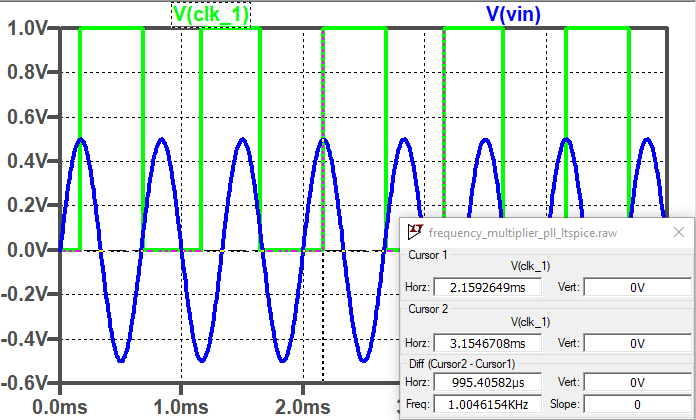
\includegraphics[width=.45\textwidth]{Fig/NoEnganche1500}
    \caption{Verde:Señal de entrada de $1,5Hz$. Azul:Señal de enganche del PLL de $1KHz$ (nodo $clk1$)}
    \label{NEsup}
\end{figure}
Al haber analizado el rangos de frecuencias de enganche del PLL para los valores $R1=50K$ y $C1=100nF$ surge la posibilidad de variar el valor del capacitor 
y ver como ésto influye en el rango de frecuencias de enganche. Para realizar esto se eligieron de forma arbitraria 3 valores de capacitores y se repitió el procedimiento anterior 
para encontrar el rango de frecuencias que el PLL sigue de forma correcta. Dando como resultado:
\begin{itemize}
    \item $C1=1nF$ $\rightarrow$ Rango de frecuencias de enganche igual a $[50Hz,1850Hz]$
    \item $C1=10nF$ $\rightarrow$ Rango de frecuencias de enganche igual a $[500Hz,1500Hz]$
    \item $C1=1000nF$ $\rightarrow$ Rango de frecuencias de enganche igual a $[990Hz,1005Hz]$
\end{itemize}
Vemos que el rango de frecuencia tiene una relación directa con el valor del capacitor.  Al aumentar la capacitancia el rango de 
engache se acota demasiado, y en cambio al disminuirla el rango de frecuencias de enganche aumenta. Siempre manteniendo fijo el 
valor de la resistencia en $50K$. Este resultado y el obtenido anteriormente al variar el valor de $R1$ nos indica lo sensible que es el circuito 
a cambios en los parametros del filtro pasa bajo, es decir que para realizar un control óptimo del PLL es fundamental analizar el valor de $\tau$ y 
ajustarlo segun el requerimiento y teniendo en cuenta como el valor $\tau$ modifica el tiempo que tarda el circuito en engancharse.\\

Por último, cambiamos la señal de entrada a nuestro circuito por una señal FM de portadora $1KHz$, con $\Delta f=300Hz$ y probando con 3 valores de señal 
moduladora: $F_m=10Hz$,$F_m=30Hz$ y $F_m=50Hz$. Al medir la señal en el nodo $Vc$ deberiamos obtener una frecuencia que coincida con la frecuencia de la moduladora, es decir 
recuperamos la moduladora de la señal FM. Los resultados obtenidos son:
\begin{itemize}
    \item $F_m=10Hz$
    \begin{figure}[H]
        \centering
        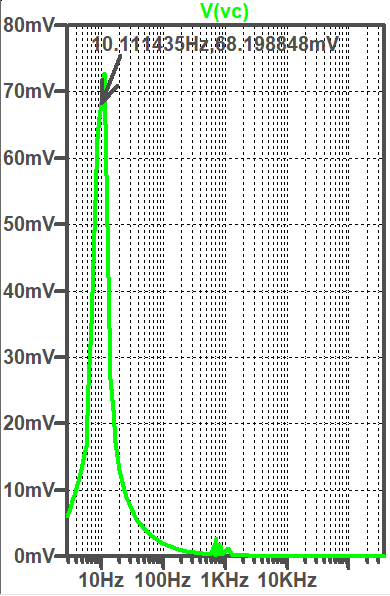
\includegraphics[width=.3\textwidth]{Fig/FFT_FMMod10Hz}
        \caption{FFT de la señal en el nodo $Vc$ evidenciando la correcta demodulación para una FM con moduladora de $10Hz$}
        \label{FM10}
    \end{figure}
    \item $F_m=30Hz$
    \begin{figure}[H]
        \centering
        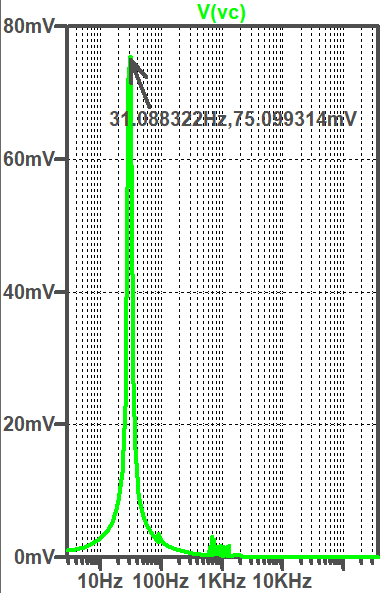
\includegraphics[width=.3\textwidth]{Fig/FFT_FMMod30Hz}
        \caption{FFT de la señal en el nodo $Vc$ evidenciando la correcta demodulación para una FM con moduladora de $30Hz$}
        \label{FM30}
    \end{figure}
    \item $F_m=50Hz$
    \begin{figure}[H]
        \centering
        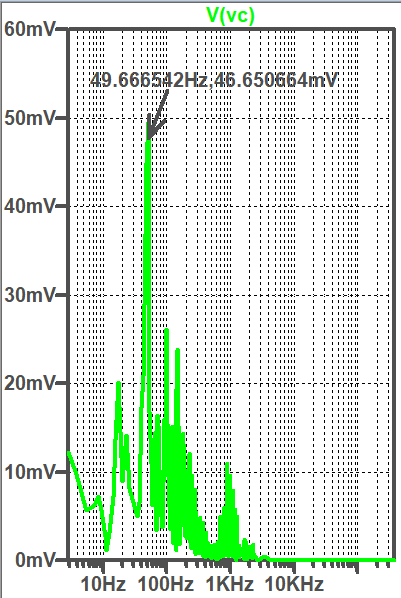
\includegraphics[width=.3\textwidth]{Fig/FFT_FMMod50Hz}
        \caption{FFT de la señal en el nodo $Vc$ evidenciando la correcta demodulación para una FM con moduladora de $50Hz$}
        \label{FM50}
    \end{figure}
\end{itemize}
Utilizando nuevamente la herramienta de la FFT que brinda el simulador, se observa que el PLL es capaz de demodular de manera 
correcta la señal FM para esos valores de frecuencia moduladora.








    
\end{document}
